\section{Experiments} 
\label{Sec:Experiments}

\subsection{Experimental Setup}

We evaluate all five methods on six NVIDIA GPUs: RTX 5090, RTX 4090, A100-PCIE-40GB, H20, H800 PCIe, and L20, under a unified software stack (Python 3.11, CUDA 11.8, PyTorch 2.10.0+cu128, Triton 3.6.0). 
All cross-machine speedups are computed against PyTorch baselines remeasured on each target machine. All performance statistics are reported over semantically correct kernels only.

\subsection{Overall Results}
\label{sec:overall_results}

Table~\ref{tab:overall-main} reveals a sharp separation across success stages: compile success, semantic correctness, and useful acceleration are distinct outcomes that do not imply one another.

Two patterns stand out.
First, a large fraction of compiled kernels remain incorrect: although 64.2\% of KernelAgent-generated kernels compile successfully, only 10.8\% are correct, yielding a Correct/Compile conversion of 16.8\%.
Second, even the strongest methods remain far from reliable. GEAK yields the highest overall correctness at only 30.7\%, while Claude yields 22.7\%.
These results motivate shifting the analysis from aggregate ranking toward understanding where and why the success frontier breaks down.

\begin{table}[t]
\centering
\small
\setlength{\tabcolsep}{7pt}
\caption{Overall results on 176 tasks. Speedup and score are averaged over correct kernels only. Correct/Compile highlights how often compiled candidates actually preserve semantics.}
\begin{tabular}{lccccc}
\toprule
Method & Compile (\%) & Correct (\%) & Correct/Compile (\%) & Speedup & Score (\%) \\
\midrule
AutoTriton  & 36.4 & 17.0 & 46.9 & 1.35 & 60.7 \\
GEAK        & 68.8 & 30.7 & 44.6 & 1.15 & 50.0 \\
KernelAgent & 64.2 & 10.8 & 16.8 & 1.41 & 68.1 \\
Claude      & 45.5 & 22.7 & 50.0 & 1.26 & 54.2 \\
KernelLLM   & 1.7  & 0.0  & 0.0  & --   & 0.0 \\
\bottomrule
\end{tabular}
\label{tab:overall-main}
\end{table}


\subsection{Correctness Is Category-Structured}
\label{sec:category_correctness}

\begin{figure*}[t]
    \centering
    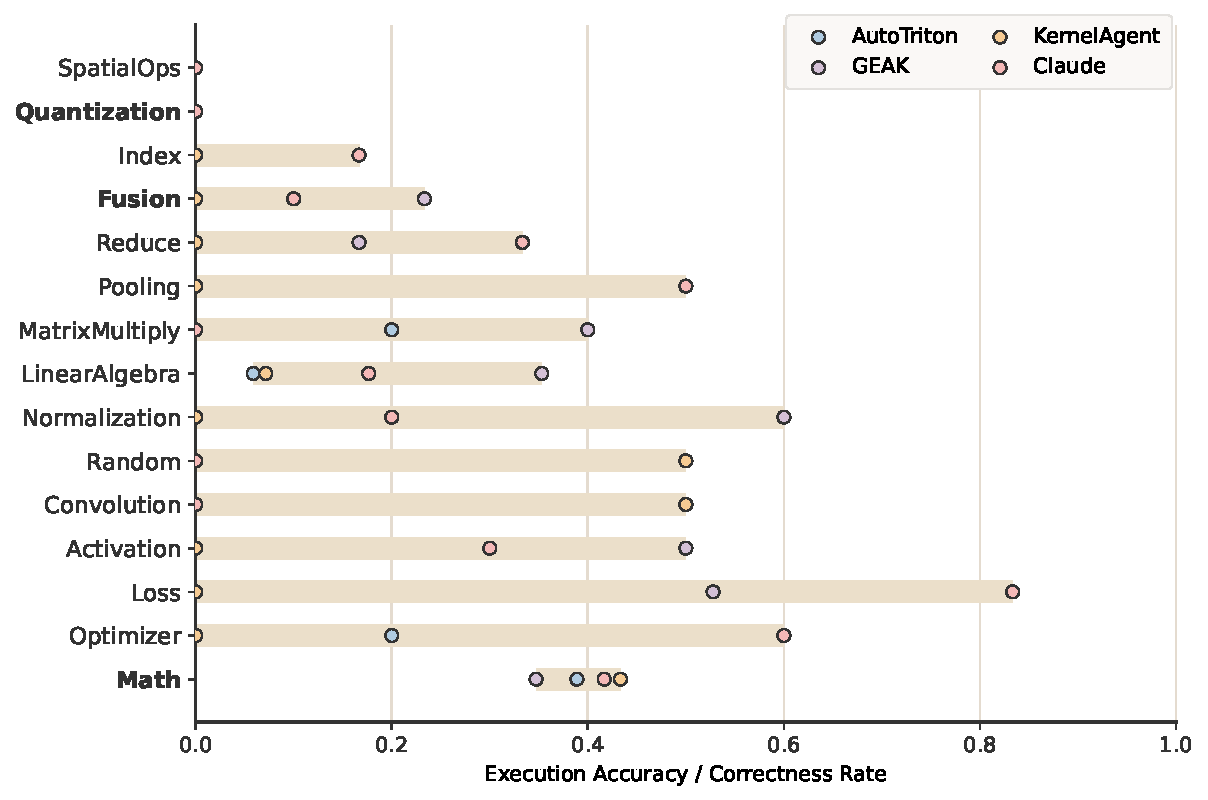
\includegraphics[width=0.88\textwidth]{src/figs/semantic_correctness_category_boundary.pdf}
    \caption{Category-Wise Correctness Across Methods.}
    \label{fig:semantic_correctness_category_boundary}
\end{figure*}

Figure~\ref{fig:semantic_correctness_category_boundary} reveals a striking pattern: correctness rates vary dramatically across categories---from near-zero in \texttt{SpatialOps} and \texttt{Quantization} to over 0.8 in \texttt{Loss}---while different methods tend to cluster within the same category band rather than separating across it. This suggests that task structure, not method identity, is the primary driver of correctness.

To quantify this, we fit task-level logistic attribution models using Pearson correlation of binary outcomes against method-indicator and category-indicator variables, reporting explained deviance as a measure of predictive power (excluding the near-zero DeepSeek-Coder baseline). Method identity and category identity explain nearly identical variance in compile success (5.18\% vs.\ 5.24\%), but for semantic correctness, category explains nearly three times more variance than method identity (9.4\% vs.\ 3.3\%). Correspondingly, adding a category on top of the method reduces deviance by 34.6, whereas adding the method on top of the category reduces it by only 13.0. While method design still matters at the executable stage, semantic correctness is primarily bounded by task structure.

Table~\ref{tab:category-conversion} further exposes where failures concentrate. Easy categories such as \texttt{Activation} and \texttt{Math} convert compiled candidates to correct kernels at rates of 46--56\%, while hard categories such as \texttt{Fusion} and \texttt{MatrixMultiply} remain near 25\%, and \texttt{Quantization} and \texttt{SpatialOps} reach 0\%.

Critically, these failures in hard categories are not caused by front-end syntax problems---their compile rates are non-trivial. To probe whether failure is instead reducible to code complexity, we compute several task-level static structure proxies and estimate their Pearson correlation with pooled correctness failure. Intermediate assignment count and fusion call count yield the strongest signal ($r \approx 0.21$), while cyclomatic complexity and a logical-span proxy yield only $r \approx 0.15$. Notably, all static proxies are more predictive of compile failure than of semantic failure. This confirms that hard-category failures represent a distinct semantic boundary, not merely harder syntax generation.


\begin{table}[t]
\centering
\caption{Representative category-level conversion from compilable code to semantically correct kernels, averaged over AutoTriton, GEAK, KernelAgent, and Claude.}
\small
\setlength{\tabcolsep}{8pt}
\begin{tabular}{lccc}
\toprule
Category & Avg. Compile (\%) & Avg. Correct (\%) & Correct/Compile (\%) \\
\midrule
Activation      & 70.0 & 32.5 & 46.4 \\
Math            & 72.2 & 40.3 & 55.8 \\
Fusion          & 43.8 & 10.8 & 24.8 \\
MatrixMultiply  & 60.0 & 15.0 & 25.0 \\
Quantization    & 41.7 & 0.0  & 0.0 \\
SpatialOps      & 25.0 & 0.0  & 0.0 \\
\bottomrule
\end{tabular}
\label{tab:category-conversion}
\end{table}



\subsection{Iterative Refinement Repairs Rather Than Optimizes}
\label{sec:iterative_refinement}

\begin{figure*}[t]
    \centering
    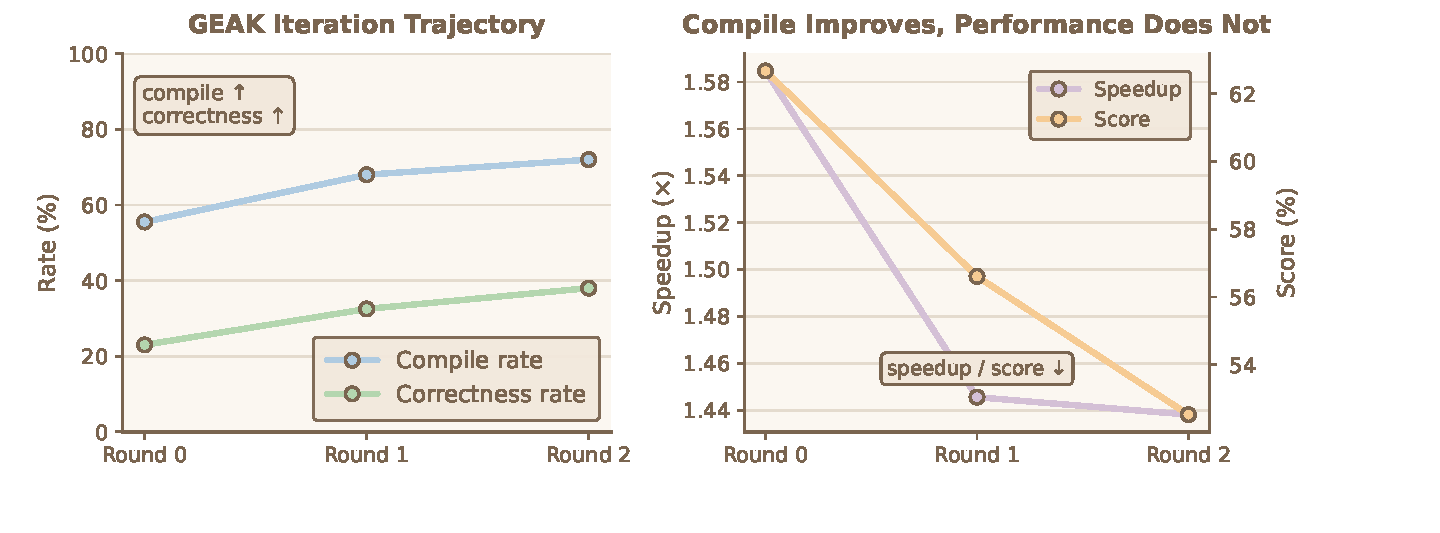
\includegraphics[width=0.90\textwidth]{src/figs/geak_iteration_trajectory.pdf}
    \caption{GEAK Iteration Trajectory.}
    \label{fig:geak_iteration_trajectory}
\end{figure*}

Figure~\ref{fig:geak_iteration_trajectory} illustrates a consistent
pattern: compile success rises from 52.3\% to 68.8\% and correctness from 18.2\%
to 30.7\%, but average speedup falls from 1.58$\times$ to 1.44$\times$ and score
from 62.7\% to 53.3\%. This performance decline will not be reversed by further iteration. KernelAgent shows the same pattern more starkly: many candidates compile, but few preserve semantics.

The performance drop is explained by the quality of newly rescued kernels. In GEAK 
rounds 0$\to$1, newly rescued correct kernels average only $1.16\times$ speedup 
(score 43.7\%), versus $1.58\times$ (score 62.9\%) for already-correct kernels. In 
rounds 1$\to$2, the gap persists: $1.32\times$ (score 35.5\%) versus $1.46\times$ 
(score 56.0\%). Analysis of 352 adjacent GEAK diffs confirms why: dominant edit 
types are no substantial change (102), mask fixes (101), delegated-op 
introduction/removal (65), and dtype/casting fixes (36), while optimization-oriented 
rewrites are rare. We analyze the structural reason for this repair bias in 
Insight~2 (\S\ref{sec:insight2}).

\subsection{High-Performance Kernel Generation Remains Challenging}

Semantic correctness is necessary, but alone insufficient for practical deployment.
Across all correct kernels, 46.6\% remain slower than eager PyTorch, and the pooled median speedup is only 1.0008$\times$. 
Cross-machine portability is also weak: the max/min speedup ratio has a median of $2.15\times$, a mean of $2.73\times$, and reaches $21.4\times$ in the worst case. Figure~\ref{fig:correct_speedup_machine_portability} shows that the fraction of correct kernels slower than PyTorch ranges from 18\% on A100 to 76\% on L20.

\begin{figure*}[t]
    \centering
    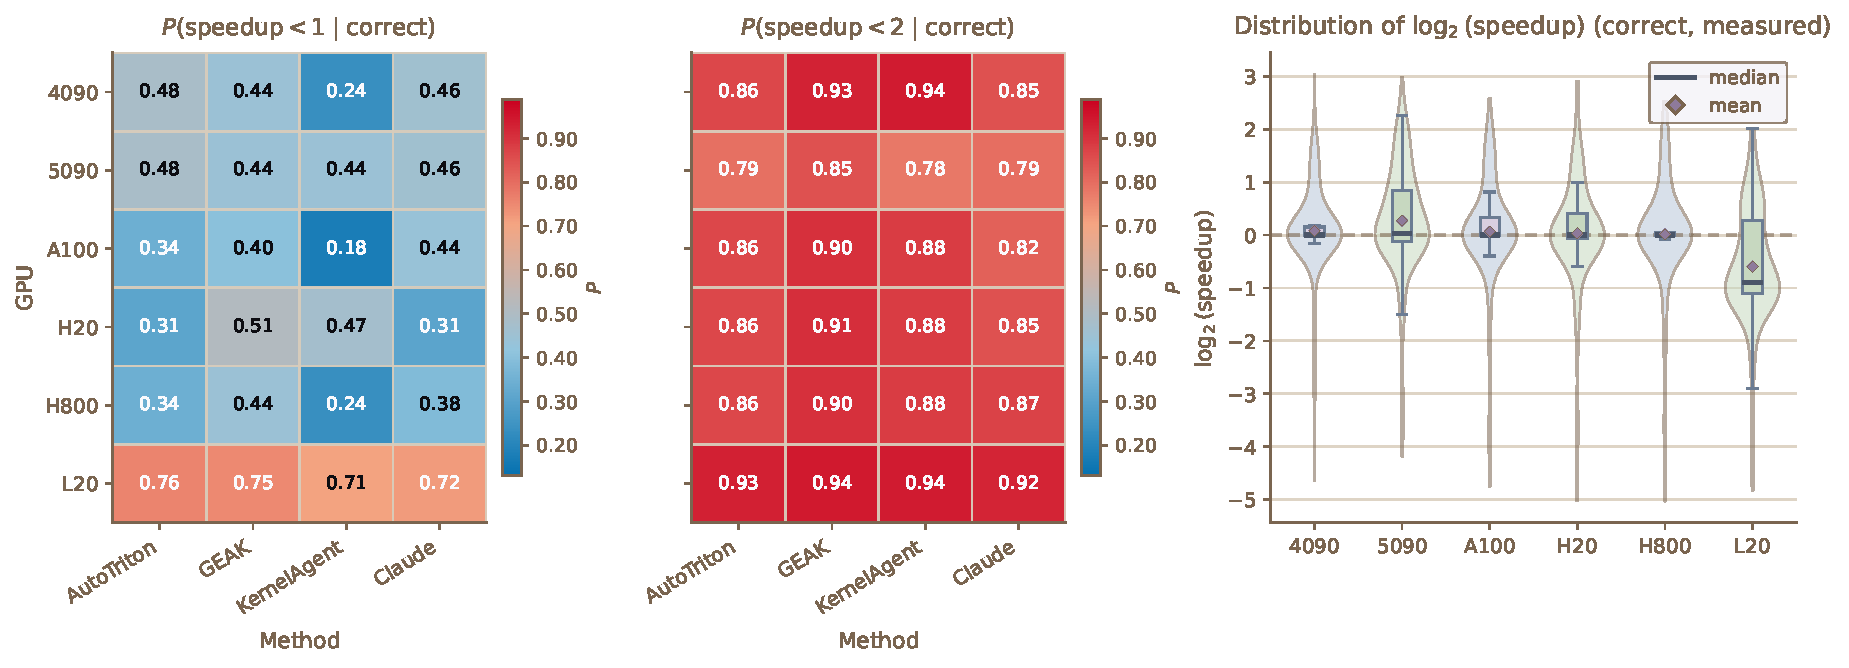
\includegraphics[width=0.97\textwidth]{src/figs/correct_speedup_machine_portability.pdf}
    \caption{Cross-hardware speedup distribution and portability of correct kernels.}
    \label{fig:correct_speedup_machine_portability}
\end{figure*}

\subsection{Case Studies}

The following cases provide mechanistic illustrations of the three findings reported 
in Section~\ref{Sec:Insights}, grounding each claim in concrete kernel-level evidence.

\subsubsection{Case 1: Local, Single-Path Semantics Define the Success Ceiling}
\label{sec:case_success}

For the \texttt{logit} task, GEAK, Claude and AutoTriton all produce correct kernels achieving approximately $3.35\times$ speedup on RTX~4090. The task is structurally minimal: each output element depends on exactly one input element, clipping is purely local, and the kernel requires neither cross-block reduction nor inter-instance coordination.
Listing~\ref{lst:logit-autotriton-4090} shows a representative implementation. GEAK and Claude produce nearly identical kernels, differing only in whether clipping uses nested \texttt{tl.where} or \texttt{tl.minimum}/\texttt{tl.maximum}.


\begin{lstlisting}[style=papercode,label={lst:logit-autotriton-4090}]
    pid = tl.program_id(0)
    offsets = pid * XBLOCK + tl.arange(0, XBLOCK)
    mask = offsets < numel
    x = tl.load(input_ptr + offsets, mask=mask)
    if eps != 0.0:
        x = tl.where(x < eps, eps, x)
        x = tl.where(x > 1.0 - eps, 1.0 - eps, x)
    logit_x = tl.math.log(x / (1.0 - x))
    tl.store(output_ptr + offsets, logit_x, mask=mask)
\end{lstlisting}

This case establishes an upper bound: when data dependence is lane-local and the implementation path is near-template, most methods are reliable.

\subsubsection{Case 2: Non-Local Semantic Composition Fails at Correctness}
\label{sec:case_global_fail}

For \texttt{fused\_exp\_mean}, GEAK generates a kernel that compiles successfully, yet produces numerically incorrect outputs. The failure is not a syntax error, but a subtle interaction among padding semantics, a nonlinear transform, and a global reduction.

\begin{lstlisting}[style=papercode]
    x = tl.load(input_ptr + offset, mask=mask, other=0.0)
    exp_x = tl.math.exp(x.to(tl.float32))
    block_sum = tl.sum(exp_x, axis=0)
    if tl.program_id(0) == 0:
        tl.store(output_ptr, 0.0)
    tl.atomic_add(output_ptr, block_sum)
\end{lstlisting}

Each local idiom is individually correct. The error arises from their composition: masked-off lanes are padded with zero \emph{before} exponentiation, causing each to contribute \texttt{exp(0)\,=\,1} rather than 0 to the global reduction. The kernel violates the contract that only valid elements should participate in the mean---a failure invisible to local testing and only detectable at the full-tensor level.

\subsubsection{Case 3: Iterative Refinement Converges to Correct but Slow Kernels}
\label{sec:case_iter}

The GEAK trajectory on \texttt{Index/expand\_where} illustrates a repair that stops at correctness. The task requires \texttt{torch.where} over three operands that must be aligned under broadcasting before the predicate is applied. Round~0 fails to compile: the generator emits indexing logic the compiler rejects. Round~1 compiles but fails correctness: execution proceeds, yet the mapping from output positions to operand elements is wrong for mixed shapes. Round~2 fixes the mapping and passes the correctness gate---but records a speedup of only $0.076{\times}$.

\begin{lstlisting}[style=papercode]
    remaining = offsets
    for dim in range(output_ndim):
        multiplier = tl.load(output_multipliers_ptr + dim)
        coord = remaining // multiplier
        remaining = remaining % multiplier
        ...
\end{lstlisting}

Iterative feedback rewards correctness but provides insufficient signal about efficiency. As a result, the surviving kernel converges to an expensive implementation that recovers broadcast coordinates via radix decomposition and performs per-axis shape and stride lookups for each operand separately.